
The ip-shuffle script embodies a systematic approach to dynamic IP address 
assignment for network interfaces in Linux and FreeBSD environments. Leveraging
Bash scripting at its core, the script orchestrates the IP address allocation 
process seamlessly. Upon execution, the program runs every 3 minutes unless the 
user wants a different runtime, the script dynamically configures essential
network parameters including the gateway, base IP, IP range, and network 
interface details, providing a flexible framework for network configuration. 
Through the utilization of dedicated functions such as
\begin{verbatim}
 generate_random_ip (), 
check_ip_availability(), 
and validate_network_config(), 
\end{verbatim}
the script ensures the
integrity and compatibility of the assigned IP addresses with the network 
infrastructure. Furthermore, the incorporation of error trapping mechanisms 
and support for common Unix signals enhances the script's reliability and r
esilience during execution, safeguarding against potential errors or 
interruptions. By adhering to modular design principles, the script maintains
flexibility and extensibility, allowing for seamless adaptation to diverse 
network configurations and environments. In essence, the ip-shuffle script 
encapsulates a robust solution for automating network interface configuration 
tasks, embodying a sophisticated yet accessible approach to dynamic IP address 
management.

\label{sec:figs}
%-------------------------------------------------------------------------------
%---------------------------


\begin{figure}
 \caption{OUR PICTURE}
  \centering
   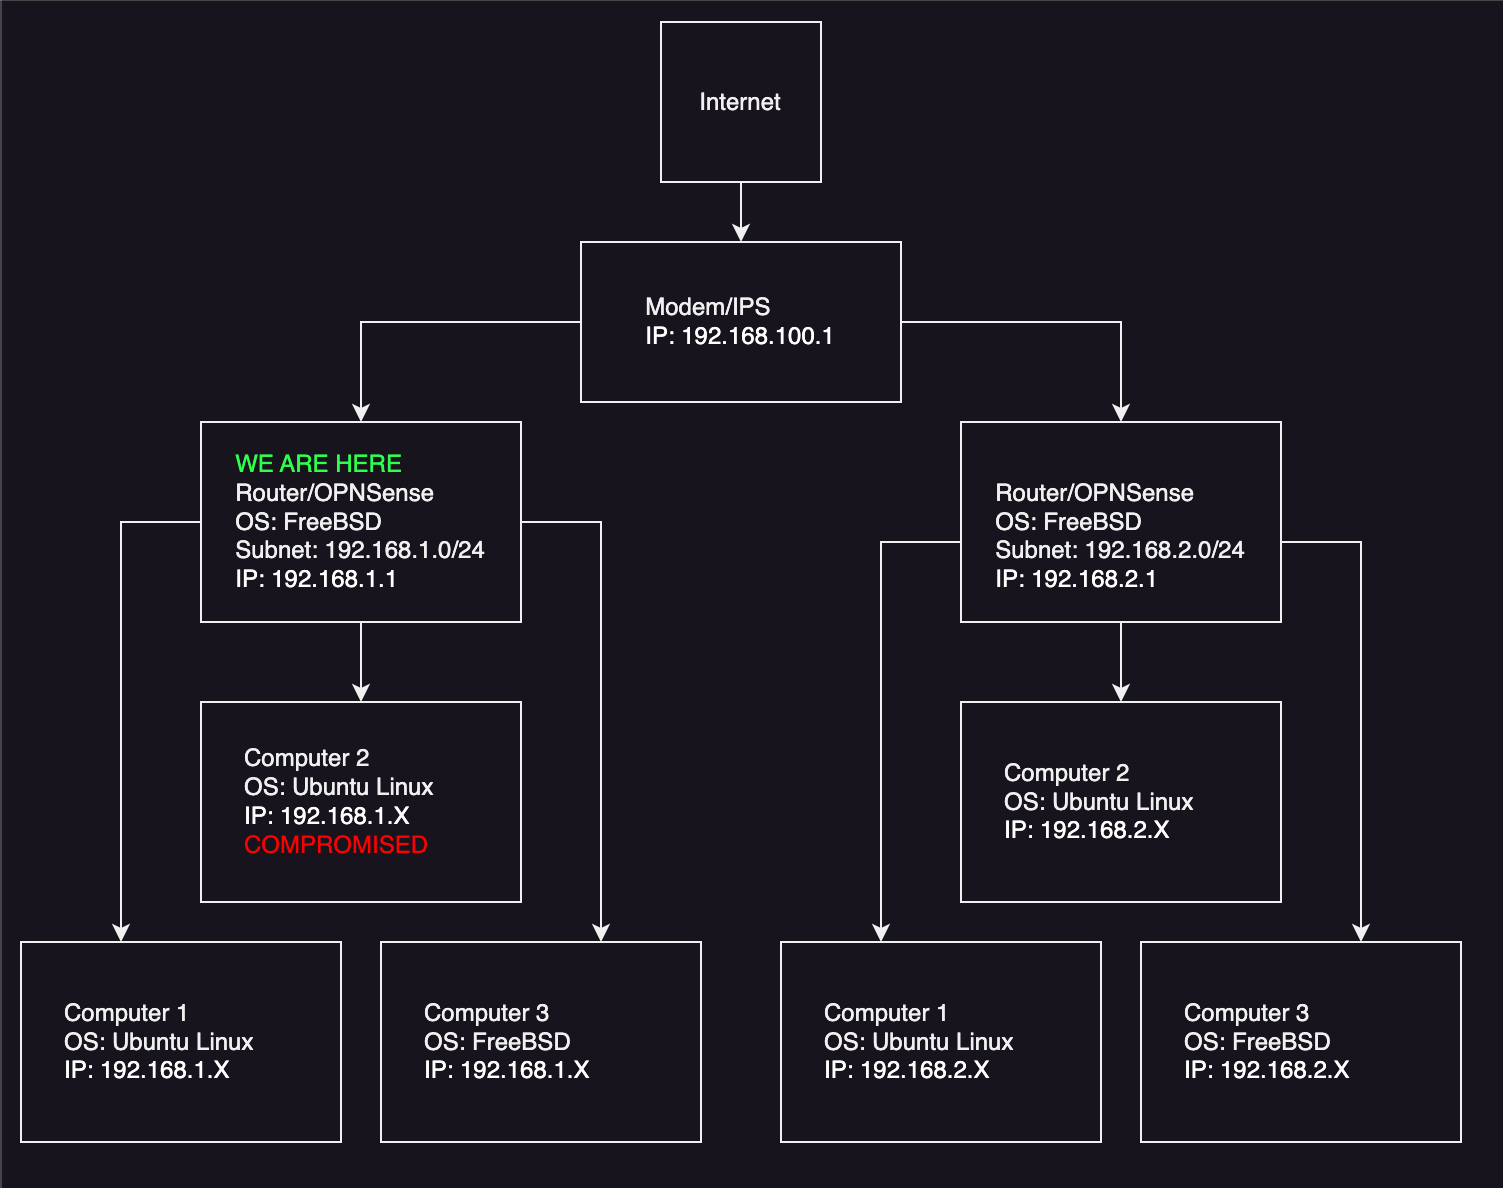
\includegraphics[width=0.5\textwidth]{diagram.jpeg}
\end{figure}

%% %---------------------------





